\graphicspath{{Figs/interpolation/}}
%
% To start the document, use
%  \chapter{...}
% For lover level, sections use
%  \section{...}
%  \subsection{...}
%
\chapter{\textindex{Interpolation}}
%-------------------------------------------------------------------------
\label{sec:interpolation}


%
% Document history, format:
%  \starthistory
%    date1 & text .... \\
%    date2 & text .... \\
%    ....
%  \stophistory
%
\starthistory
  100204 & Added documentation of grid checking functions by Stefan Buehler.\\
  020528 & Created by Stefan Buehler.\\
\stophistory




%
% Introduction
%

There are no general single-step interpolation functions in ARTS.
Instead, there is a set of useful utility functions that can be used
to achieve interpolation. Roughly, you can separate these into
functions determining grid position arrays, functions determining
interpolation weight tensors, and functions applying the
interpolation. Doing an interpolation thus requires a chain of
function calls:
\begin{enumerate}
\item \funcindex{gridpos} (one for each interpolation dimension)
\item \funcindex{interpweights}
\item \funcindex{interp}
\end{enumerate}
Currently implemented in ARTS is mulitlinear interpolation in up to 6
dimensions. (Is the 6D case called hexa-linear interpolation?)  The
necessary functions and their interaction will be explained in this
chapter.

\section{Implementation files}
%-------------------------------------------------------------------------

Variables and functions related to interpolation are defined in the files:
\begin{itemize}
\item \fileindex{interpolation.h}
\item \fileindex{interpolation.cc}
\item \fileindex{test\_interpolation.cc}
\end{itemize}
The first two files contain the declarations and implementation, the
last file some usage examples.

\section{Green and blue interpolation}
%-------------------------------------------------------------------------

\begin{figure}[htbp]
  \centering
  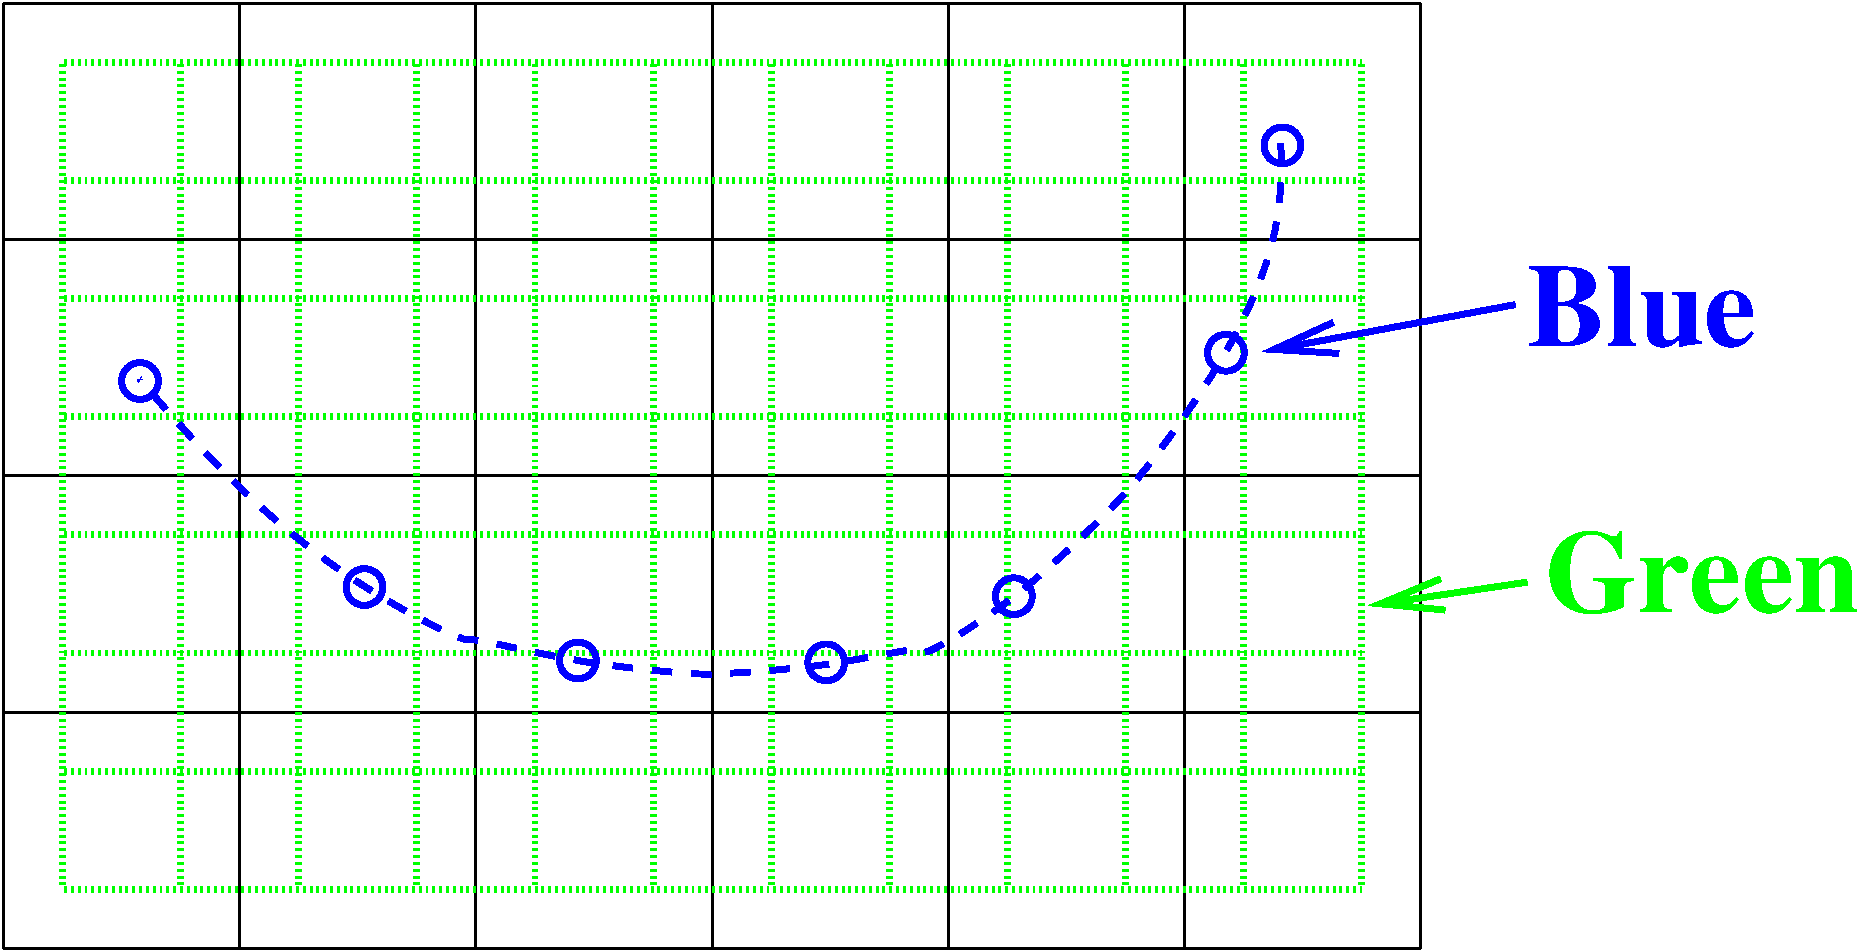
\includegraphics[width=.6\hsize]{interpolation_types}
  \caption{The two different types of interpolation. Green (dotted):
    Interpolation to a new grid, output has same dimension as input,
    in this case 2D. Blue (dashed): Interpolation to a sequence of
    points, output is always 1D.}
  \label{fig:interpolation:types}
\end{figure}

There are two different types of interpolation in ARTS:
\begin{description}
\item[\textindex{Green Interpolation}:] Interpolation of a gridded field to a new
  grid.
\item[\textindex{Blue Interpolation}:] Interpolation of a gridded field to a
  sequence of positions.
\end{description}
Figure \ref{fig:interpolation:types} illustrates the different types
for a 2D example. 

The first step of an interpolation always consists in determining
where your new points are, relative to the original grid. You can do
this separately for each dimension. The positions have to be stored
somehow, which is described in the next section.

\section{Grid checking functions}
%-------------------------------------------------------------------------
\label{sec:interpolation:gridchecking}

Before you do an interpolation, you should check that the new grid is
inside the old grid. (Or only slightly outside.) You can use the
convenient function \funcindex{chk\_interpolation\_grids} for this
purpose, which resides in file \fileindex{check\_input.cc}. The
function has the following parameters:

{\small
\begin{verbatim}
const String&     which_interpolation   A string describing the 
                                        interpolation for which 
                                        the grids are intended. 
ConstVectorView   old_grid              The original grid.
ConstVectorView   new_grid              The new grid.
const Numeric&    extpolfac             The extrapolation fraction. 
                                        See gridpos function for 
                                        details. Has a default 
                                        value, which is consistent 
                                        with gridpos.  
\end{verbatim}
}

There is also a special version for the case that the new grid is just
a scalar. What the function does is check if old and new grid for an
interpolation are ok. If not, it throws a detailed runtime error
message. 

The parameter \artsstyle{extpolfac} determines how much extrapolation
is tolerated. Its default value is 0.5, which means that we allow
extrapolation as far out as half the spacing of the last two grid
points on that edge of the grid.

The \artsstyle{chk\_interpolation\_grids} function is quite thorough.
It checks not only the grid range, but also the proper sorting,
whether there are duplicate values, etc.. It is not completely cheap
computationally. Its intended use is at the beginning of workspace
methods, when you check the input variables and issue runtime errors
if there are any problems. The runtime error thrown also explains in
quite a lot of detail what is actually wrong with the grids.
  

\section{Grid positions}
%-------------------------------------------------------------------------
\label{sec:interpolation:gridpos}

A grid position specifies where an interpolation point is, relative
to the original grid. It consists of three parts, an \artsstyle{Index} giving the
original grid index below the interpolation point, a \artsstyle{Numeric}
giving the fractional distance to the next original grid point, and a
\artsstyle{Numeric} giving 1 minus this number. Of course, the last element is
redundant. However, it is efficient to store this, since it is used
many times over. We store the two numerics in a plain C array of
dimension 2. (No need to use a fancy Array or Vector for this, since
the dimension is fixed.) So the structure \typeindex{GridPos} looks like:

\begin{verbatim}
struct GridPos  {
   Index   idx;      /*!< Original grid index below
                          interpolation point. */
   Numeric fd[2];    /*!< Fractional distance to next point
                          (0<=fd[0]<=1), fd[1] = 1-fd[0]. */ 
};
\end{verbatim}

For example, \artsstyle{idx}=3 and \artsstyle{fd}=0.5 means that this interpolation point is
half-way between index 3 and 4 of the original grid.  Note, that
`below' in the first paragraph means `with a lower index'. If the
original grid is sorted in descending order, the value at the grid
point below the interpolation point will be numerically higher than
the interpolation point.  In other words, grid positions and
fractional distances are defined relative to the order of the original
grid. Examples:

{\small
\begin{verbatim}
old grid = 2 3
new grid = 2.25
idx      = 0
fd[0]    = 0.25

old grid = 3 2
new grid = 2.25
idx      = 0
fd[0]    = 0.75
\end{verbatim}
}

Note that \artsstyle{fd[0]} is different in the second case, because the old grid
is sorted in descending order. Note also that \artsstyle{idx} is the same in
both cases.

Grid positions for a whole new grid are stored in an \artsstyle{Array<GridPos>}
(called \artsstyle{ArrayOfGridPos}). 

\section{Setting up grid position arrays}
%----------------------------------------------------------------------

There is only one function to set up grid position arrays, namely 
\funcindex{gridpos}:

{\small
\begin{verbatim}
void gridpos( ArrayOfGridPos& gp,
              ConstVectorView old_grid,
              ConstVectorView new_grid 
              const Numeric&  extpolfac=0.5 );
\end{verbatim}
}

\hspace{-\parindent}Some points to remember:
\begin{itemize}
\item As usual, the output \artsstyle{gp} has to have the right dimension. 
  
\item The old grid has to be strictly sorted. It can be in ascending
  or descending order. But there must not be any duplicate values.
  Furthermore, the old grid must contain at least two points.
  
\item   The new grid does not have to be sorted, but the function will be
  faster if it is sorted or mostly sorted. It is ok if the new grid
  contains only one point.
  
\item   The beauty is, that this is all it needs to do also interpolation in
  higher dimensions: You just have to call gridpos for all the
  dimensions that you want to interpolate.
  
\item   Note also, that for this step you do not need the field itself at
  all!

\item   Finally, note that parameter \artsstyle{extpolfac} plays the
  same role as explained above in Section
  \ref{sec:interpolation:gridchecking}. 
\end{itemize}

\section{\textindex{Interpolation weights}}
%----------------------------------------------------------------------

As explained in the `Numerical Recipes'
\citep{numerical_recipes_C:97}, 2D bi-linear interpolation means, that
the interpolated value is a weighted average of the original field at
the four corner points of the grid square in which the interpolation
point is located. For simplicity, we label the four corner points
counterclockwise, starting from the lower left point (Figure
\ref{fig:interpolation:square}).  Then the interpolated value is given
by:
\begin{eqnarray}
  y(t,u)
  &=& (1-t)*(1-u)*y_1 \nonumber \\
  & & \mbox{} + t*(1-u)*y_2 \nonumber \\
  & & \mbox{} + t*u*y_3 \nonumber \\
  & & \mbox{} + (1-t)*u*y_4 \nonumber \\
  &=& w_1*y_1 + w_2*y_2 + w_3*y_3 + w_4*y_4
\label{eq:interpolation:weights}
\end{eqnarray}
where $t$ and $u$ are the fractional distances between the
corner points in the two dimensions, $y_i$ are the field values
at the corner points, and $w_i$ are the interpolation weights.

\begin{figure}
  \centering
  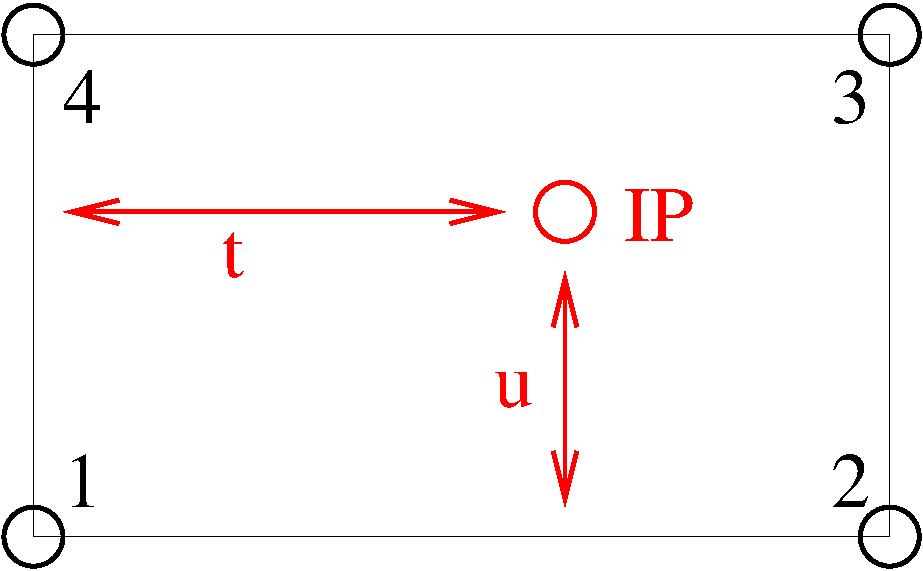
\includegraphics[width=.4\hsize]{interpolation_square}
  \caption{The grid square for 2D interpolation. The numbers 1\ldots 4
    mark the corner points, IP is the interpolation point, $t$ and $u$
    are the fractional distances in the two dimensions.}
  \label{fig:interpolation:square}
\end{figure}

(By the way, I have discovered that this is exactly the result that
you get if you first interpolate linearly in one dimension, then in
the other. I was playing around with this a bit, but it is the more
efficient way to pre-calculate the $w_i$ and do all dimensions at once.

How many interpolation weights one needs for a multilinear
interpolation depends on the dimension of the interpolation: There are
exactly $2^n$ interpolation weights for an $n$ dimensional
interpolation.  These weights have have to be computed for each
interpolation point (each grid point of the new grid, if we do a
`green' type interpolation. Or each point in the sequence, if we do a
`blue' type interpolation).

This means, calculating the interpolation weights is not exactly
cheap, especially if one interpolates simultaneously in many
dimensions. On the other hand, one can save a lot by re-using the
weights.  Therefore, interpolation weights in ARTS are stored in a
tensor which has one more dimension than the output field. The last
dimension is for the weight, so this last dimension has the extent 4
in the 2D case, 8 in the 3D case, and so on (always $2^n$).

In the case of a `blue' type interpolation, the weights are
always stored in a matrix, since the output field is always 1D (a
vector). 

\section{Setting up interpolation weight tensors}
%----------------------------------------------------------------------

Interpolation weight tensors can be computed by a family of functions,
which are all called \funcindex{interpweights}. Which function is actually
used depends on the dimension of the input and output quantities. For
this step we still do not need the actual fields, just the grid
positions.

\subsection{Blue interpolation}

In this case the functions are:

{\small
\begin{verbatim}
void interpweights( MatrixView itw,
                    const ArrayOfGridPos& cgp );
void interpweights( MatrixView itw,
                    const ArrayOfGridPos& rgp,
                    const ArrayOfGridPos& cgp );
void interpweights( MatrixView itw,
                    const ArrayOfGridPos& pgp,
                    const ArrayOfGridPos& rgp,
                    const ArrayOfGridPos& cgp );
void interpweights( MatrixView itw,
                    const ArrayOfGridPos& vgp,
                    const ArrayOfGridPos& sgp,
                    const ArrayOfGridPos& bgp,
                    const ArrayOfGridPos& pgp,
                    const ArrayOfGridPos& rgp,
                    const ArrayOfGridPos& cgp );
\end{verbatim}
}

In all cases, the dimension of \artsstyle{itw} must be consistent with the
given grid position arrays and the dimension of the interpolation
(last dimension $2^n$). Because the grid position arrays are
interpreted as defining a sequence of positions they must all have
the same length.

\subsection{Green interpolation}

In this case the functions are:

{\small
\begin{verbatim}
void interpweights( Tensor3View itw,
                    const ArrayOfGridPos& rgp,
                    const ArrayOfGridPos& cgp );
void interpweights( Tensor4View itw,
                    const ArrayOfGridPos& pgp,
                    const ArrayOfGridPos& rgp,
                    const ArrayOfGridPos& cgp );
void interpweights( Tensor5View itw,
                    const ArrayOfGridPos& bgp,
                    const ArrayOfGridPos& pgp,
                    const ArrayOfGridPos& rgp,
                    const ArrayOfGridPos& cgp );
void interpweights( Tensor6View itw,
                    const ArrayOfGridPos& sgp,
                    const ArrayOfGridPos& bgp,
                    const ArrayOfGridPos& pgp,
                    const ArrayOfGridPos& rgp,
                    const ArrayOfGridPos& cgp );
void interpweights( Tensor7View itw,
                    const ArrayOfGridPos& vgp,
                    const ArrayOfGridPos& sgp,
                    const ArrayOfGridPos& bgp,
                    const ArrayOfGridPos& pgp,
                    const ArrayOfGridPos& rgp,
                    const ArrayOfGridPos& cgp );
\end{verbatim}
}

In this case the grid position arrays are interpreted as defining the
grids for the interpolated field, therefore they can have different
lengths. Of course, \artsstyle{itw} must be consistent with the length of
all the grid position arrays, and with the dimension of the
interpolation (last dimension $2^n$).

\section{The actual interpolation}
%----------------------------------------------------------------------

For this final step we need the grid positions, the
interpolation weights, and the actual fields. For each interpolated
value, the weights are applied to the appropriate original field values
and the sum is taken (see Equation
\ref{eq:interpolation:weights}). The \funcindex{interp} family of functions
performs this step.

\subsection{Blue interpolation}

{\small
\begin{verbatim}
void interp( VectorView            ia,
             ConstMatrixView       itw,
             ConstVectorView       a,    
             const ArrayOfGridPos& cgp);
void interp( VectorView            ia,
             ConstMatrixView       itw,
             ConstMatrixView       a,    
             const ArrayOfGridPos& rgp,
             const ArrayOfGridPos& cgp);
void interp( VectorView            ia,
             ConstMatrixView       itw,
             ConstTensor3View      a,    
             const ArrayOfGridPos& pgp,
             const ArrayOfGridPos& rgp,
             const ArrayOfGridPos& cgp);
void interp( VectorView            ia,
             ConstMatrixView       itw,
             ConstTensor4View      a,    
             const ArrayOfGridPos& bgp,
             const ArrayOfGridPos& pgp,
             const ArrayOfGridPos& rgp,
             const ArrayOfGridPos& cgp);
void interp( VectorView            ia,
             ConstMatrixView       itw,
             ConstTensor5View      a,    
             const ArrayOfGridPos& sgp,
             const ArrayOfGridPos& bgp,
             const ArrayOfGridPos& pgp,
             const ArrayOfGridPos& rgp,
             const ArrayOfGridPos& cgp);
void interp( VectorView            ia,
             ConstMatrixView       itw,
             ConstTensor6View      a,    
             const ArrayOfGridPos& vgp,
             const ArrayOfGridPos& sgp,
             const ArrayOfGridPos& bgp,
             const ArrayOfGridPos& pgp,
             const ArrayOfGridPos& rgp,
             const ArrayOfGridPos& cgp);
\end{verbatim}
}

\subsection{Green interpolation}

{\small
\begin{verbatim}
void interp( MatrixView            ia,
             ConstTensor3View      itw,
             ConstMatrixView       a,   
             const ArrayOfGridPos& rgp,
             const ArrayOfGridPos& cgp);
void interp( Tensor3View           ia,
             ConstTensor4View      itw,
             ConstTensor3View      a,   
             const ArrayOfGridPos& pgp,
             const ArrayOfGridPos& rgp,
             const ArrayOfGridPos& cgp);
void interp( Tensor4View           ia,
             ConstTensor5View      itw,
             ConstTensor4View      a,   
             const ArrayOfGridPos& bgp,
             const ArrayOfGridPos& pgp,
             const ArrayOfGridPos& rgp,
             const ArrayOfGridPos& cgp);
void interp( Tensor5View           ia,
             ConstTensor6View      itw,
             ConstTensor5View      a,   
             const ArrayOfGridPos& sgp,
             const ArrayOfGridPos& bgp,
             const ArrayOfGridPos& pgp,
             const ArrayOfGridPos& rgp,
             const ArrayOfGridPos& cgp);
void interp( Tensor6View           ia,
             ConstTensor7View      itw,
             ConstTensor6View      a,   
             const ArrayOfGridPos& vgp,
             const ArrayOfGridPos& sgp,
             const ArrayOfGridPos& bgp,
             const ArrayOfGridPos& pgp,
             const ArrayOfGridPos& rgp,
             const ArrayOfGridPos& cgp);
\end{verbatim}
}

\section{Examples}
%----------------------------------------------------------------------

\subsection{A simple example}

This example is contained in file \fileindex{test\_interpolation.cc}.

{\small
\begin{verbatim}
void test05()
{
  cout << "Very simple interpolation case\n";

  Vector og(1,5,+1);            // 1, 2, 3, 4, 5
  Vector ng(2,5,0.25);          // 2.0, 2,25, 2.5, 2.75, 3.0

  cout << "Original grid:\n" << og << "\n";
  cout << "New grid:\n" << ng << "\n";

  // To store the grid positions:
  ArrayOfGridPos gp(ng.nelem());

  gridpos(gp,og,ng);
  cout << "Grid positions:\n" << gp;

  // To store interpolation weights:
  Matrix itw(gp.nelem(),2);
  interpweights(itw,gp);
    
  cout << "Interpolation weights:\n" << itw << "\n";

  // Original field:
  Vector of(og.nelem(),0);
  of[2] = 10;                   // 0, 0, 10, 0, 0

  cout << "Original field:\n" << of << "\n";

  // Interpolated field:
  Vector nf(ng.nelem());

  interp(nf, itw, of, gp);

  cout << "New field:\n" << nf << "\n";
}
\end{verbatim}
}

\hspace{-\parindent}Ok, maybe you think this is not so simple, but a
large part of the code is either setting up the example grids and
fields, or output. And here is how the output looks like:

{\small
\begin{verbatim}
Very simple interpolation case
Original grid:
  1   2   3   4   5
New grid:
  2 2.25 2.5 2.75   3
Grid positions:
   1 0    1
   1 0.25 0.75
   1 0.5  0.5
   1 0.75 0.25
   1 1    0
Interpolation weights:
  1   0
0.75 0.25
0.5 0.5
0.25 0.75
  0   1
Original field:
  0   0  10   0   0
New field:
  0 2.5   5 7.5  10
\end{verbatim}
}

\subsection{A more elaborate example}

What if you want to interpolate only some dimensions of a tensor,
while retaining others? --- You have to make a loop yourself, but it
is very easy. Below is an explicit example for a more complicated
interpolation case. (Green type interpolation of all pages of a
Tensor3.) This example is also contained in file
\artsstyle{test\_interpolation.cc}.

{\small
\begin{verbatim}
void test04()
{
  cout << "Green type interpolation of all "
       << "pages of a Tensor3\n";

  // The original Tensor is called a, the new one n. 

  // 10 pages, 20 rows, 30 columns, all grids are: 1,2,3
  Vector  a_pgrid(1,3,1), a_rgrid(1,3,1), a_cgrid(1,3,1); 
  Tensor3 a( a_pgrid.nelem(),
             a_rgrid.nelem(),
             a_cgrid.nelem() ); 
  a = 0;
  // Put some simple numbers in the middle of each page:
  a(0,1,1) = 10;
  a(1,1,1) = 20;
  a(2,1,1) = 30;

  // New row and column grids:
  // 1, 1.5, 2, 2.5, 3
  Vector  n_rgrid(1,5,.5), n_cgrid(1,5,.5); 
  Tensor3 n( a_pgrid.nelem(),
             n_rgrid.nelem(),
             n_cgrid.nelem() ); 

  // So, n has the same number of pages as a, 
  // but more rows and columns.

  // Get the grid position arrays:
  ArrayOfGridPos n_rgp(n_rgrid.nelem()); // For rows.
  ArrayOfGridPos n_cgp(n_cgrid.nelem()); // For columns.

  gridpos( n_rgp, a_rgrid, n_rgrid );
  gridpos( n_cgp, a_cgrid, n_cgrid );

  // Get the interpolation weights:
  Tensor3 itw( n_rgrid.nelem(), n_cgrid.nelem(), 4 );
  interpweights( itw, n_rgp, n_cgp );

  // Do a "green" interpolation for all pages of a:

  for ( Index i=0; i<a.npages(); ++i )
    {
      // Select the current page of both a and n:
      ConstMatrixView ap = a( i,
                              Range(joker), Range(joker) );
      MatrixView      np = n( i,
                              Range(joker), Range(joker) );

      // Do the interpolation:
      interp( np, itw, ap, n_rgp, n_cgp );

      // Note that this is efficient, because interpolation
      // weights and grid positions are re-used.
    }

  cout << "Original field:\n";
  for ( Index i=0; i<a.npages(); ++i )
      cout << "page " << i << ":\n"
           << a(i,Range(joker),Range(joker)) << "\n";

  cout << "Interpolated field:\n";
  for ( Index i=0; i<n.npages(); ++i )
      cout << "page " << i << ":\n"
           << n(i,Range(joker),Range(joker)) << "\n";
}
\end{verbatim}
}

\hspace{-\parindent}The output is:

{\small
\begin{verbatim}
Green type interpolation of all pages of a Tensor3
Original field:
page 0:
  0   0   0
  0  10   0
  0   0   0
page 1:
  0   0   0
  0  20   0
  0   0   0
page 2:
  0   0   0
  0  30   0
  0   0   0
Interpolated field:
page 0:
  0   0   0   0   0
  0 2.5   5 2.5   0
  0   5  10   5   0
  0 2.5   5 2.5   0
  0   0   0   0   0
page 1:
  0   0   0   0   0
  0   5  10   5   0
  0  10  20  10   0
  0   5  10   5   0
  0   0   0   0   0
page 2:
  0   0   0   0   0
  0 7.5  15 7.5   0
  0  15  30  15   0
  0 7.5  15 7.5   0
  0   0   0   0   0
\end{verbatim}
}


\section{Higher order interpolation}
%----------------------------------------------------------------------

Everything that was written so far in this chapter referred to linear
interpolation, which uses 2 neighboring data points in the 1D
case. But ARTS has also a framework for higher order polynomial
interpolation. It is defined in the two files

\begin{itemize}
\item \artsstyle{interpolation\_poly.h}
\item \artsstyle{interpolation\_poly.cc}
\end{itemize}

We define interpolation order $O$ as the order of the polynomial that
is used. Linear interpolation, the ARTS standard case, corresponds to
$O=1$. $O=2$ is quadratic interpolation, $O=3$ cubic interpolation.
The number of interpolation points (and weights) for a 1D
interpolation is $O+1$ for each point in the new grid. So, linear
interpolation uses 2 points, quadratic 3, and cubic 4.

Note, that if you use even interpolation orders, you will have an
unequal number of interpolation points `to the left' and `to the
right' of your new point. This is an argument for preferring $O=3$ as the
basic higher order polynomial interpolation, instead of $O=2$.

Overall, higher order interpolation works rather similarly to the
linear case.  The main difference is that grid positions for higher
order interpolation are stored in an object of type
\artsstyle{GridPosPoly}, instead of \artsstyle{GridPos}. A
\artsstyle{GridPosPoly} object contains grid indices and interpolation
weights for all interpolation points. For each point in the new grid,
there are $O+1$ indices and $O+1$ weights.

The reason
why we store all interpolation point indices, and not only the index
of the first point, is to allow correct handling of circular
interpolation, for example in scattering phase function $\phi$
angle. If the angle goes from 0 to 360$^\circ$, then points just below
360 should be used in interpolations to points just above 0, so the
indices to use are not contiguous in memory. Functions to handle this
are not yet implemented, but this should be a relatively simple matter.

In contrast to \artsstyle{GridPos}, \artsstyle{GridPosPoly} stores
weights \artsstyle{w} rather than fractional distances \artsstyle{fd}.
For the linear case:
\begin{verbatim}
  w[0] = fd[1]
  w[1] = fd[0]
\end{verbatim}

So the two concepts are almost the same.  Because the w are associated
with each interpolation point, they work also for higher interpolation
order, whereas the concept of fractional distance does not.

The weights are calculated according to 
section 3.1, eq. 3.1.1 of \citep{numerical_recipes_C:97}. These are
for the 1D case. For 2D and higher dimensional cases, the weights of
the individual dimensions have to be multiplied, just as in the linear
interpolation case.

Instead of \artsstyle{gridpos}, you have to use the function
\artsstyle{gridpos\_poly} for higher order interpolation. It works
exactly like \artsstyle{gridpos}, but has an additional argument that
gives the interpolation order $O$. 

After setting up the \artsstyle{GridPosPoly} object with
\artsstyle{gridpos\_poly}, you have to call \artsstyle{interpweights}
and \artsstyle{interp}, exactly as in the linear case. (The actual
functions used are not the same, since the name is overloaded. The
\artsstyle{interpweights} and \artsstyle{interp} functions for use
with \artsstyle{GridPosPoly} are implemented in
\artsstyle{interpolation\_poly.cc}.) So, a complete interpolation chain
involves:

\begin{verbatim}
gridpos_poly
interpweights
interp
\end{verbatim}

For $O=1$ the result of the
interpolation chain will be the same as for the linear interpolation
routines. Below is a simple complete example, taken from
the file \artsstyle{test\_interpolation.cc} in the arts source directory: 

\begin{verbatim}
void test08()
{
  cout << "Very simple interpolation case for the "
       << "new higher order polynomials.\n";

  Vector og(1,5,+1);            // 1, 2, 3, 4, 5
  Vector ng(2,5,0.25);          // 2.0, 2,25, 2.5, 2.75, 3.0

  cout << "Original grid:\n" << og << "\n";
  cout << "New grid:\n" << ng << "\n";

  // To store the grid positions:
  ArrayOfGridPosPoly gp(ng.nelem());

  Index order=2;                // Interpolation order.

  gridpos_poly(gp,og,ng,order);
  cout << "Grid positions:\n" << gp;

  // To store interpolation weights:
  Matrix itw(gp.nelem(),order+1);
  interpweights(itw,gp);
    
  cout << "Interpolation weights:\n" << itw << "\n";

  // Original field:
  Vector of(og.nelem(),0);
  of[2] = 10;                   // 0, 0, 10, 0, 0

  cout << "Original field:\n" << of << "\n";

  // Interpolated field:
  Vector nf(ng.nelem());

  interp(nf, itw, of, gp);

  cout << "New field (order=" << order << "):\n" << nf << "\n";  

  cout << "All orders systematically:\n";
  for (order=1; order<5; ++order)
    {
      gridpos_poly(gp,og,ng,order);
      itw.resize(gp.nelem(),order+1);
      interpweights(itw,gp);
      interp(nf, itw, of, gp);

      cout << "order " << order << ": ";
      for (Index i=0; i<nf.nelem(); ++i)
        cout << setw(8) << nf[i] << " ";
      cout << "\n";
    }
}
\end{verbatim}



\section{Summary}
%----------------------------------------------------------------------

Now you probably understand better what was written at the very
beginning of this chapter, namely that doing an interpolation always
requires the chain of function calls:
\begin{enumerate}
\item \artsstyle{gridpos} or \artsstyle{gridpos\_poly} (one for each interpolation dimension)
\item \artsstyle{interpweights}
\item \artsstyle{interp}
\end{enumerate}
If you are interested in how the functions really work, look in file
\artsstyle{interpolation.cc} or \artsstyle{interpolation\_poly.cc}.
The documentation there is quite detailed.  When you are using
interpolation, you should always give some thought to whether you can
re-use grid positions or even interpolation weights. This can really
save you a lot of computation time. For example, if you want to
interpolate several fields --- which are all on the same grids --- to
some position, you only have to compute the weights once.


%%% Local Variables: 
%%% mode: latex 
%%% TeX-master: "uguide" 
%%% TeX-master: "uguide"
%%% End:

